\begin{ex}
(Vunesp) Dispomos de 4 cores para pintar o mapa esquematizado na figura, com os países P, Q, R e S, de modo que países cuja fronteira comum é uma linha não podem ser coloridos com a mesma cor. De quantas maneiras é possível colorir o mapa, se:
   \begin{enumerate}[(a)]
   \item P e S forem coloridos com cores diferentes?
   \item P e S forem coloridos com a mesma cor?
   \end{enumerate}
\begin{center}
   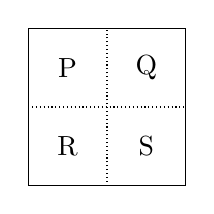
\begin{tikzpicture}
   \draw (0,0)--(2,0)--(2,2)--(0,2)--(0,0);
   \draw [densely dotted] (0,1)-- (2,1);
   \draw [densely dotted] (1,0)--(1,2);
   \draw node at (.5,.5)  {R};
   \draw node at (.5,1.5) {P};
   \draw node at (1.5,.5) {S};
   \draw node at (1.5,1.5) {Q};
   
   \end{tikzpicture}
\end{center}
 \begin{sol}
   \phantom{A} 
    \begin{enumerate} [(a)]
        \item $4\cdot3\cdot2\cdot2=48$
        \item $4\cdot1\cdot3\cdot3=36$
    \end{enumerate}
 \end{sol}

\end{ex}